% !TeX root = RJwrapper.tex
\title{Computer Algebra in R Bridges a Gap Between Symbolic Mathematics and Data in the Teaching of Statistics and Data Science}


\author{by Mikkel Meyer Andersen and Søren Højsgaard}

\maketitle

\abstract{%
The capability of R to do symbolic mathematics is enhanced by the reticulate and caracas packages. The workhorse behind these packages is the Python computer algebra library SymPy. Via reticulate, the SymPy library can be accessed from within R. This, however, requires some knowledge of SymPy, Python and reticulate. The caracas package, on the other hand, provides access to SymPy (via reticulate) but by using R syntax, and this is the main contribution of caracas. We show examples of how to use the SymPy library from R via reticulate and caracas. Using caracas, we demonstrate how mathematics and statistics can benefit from bridging computer algebra and data via R. The caracas package integrates well with Rmarkdown and Quarto, and as such supports creation of teaching material and scientific reports. As inspiration for teachers, we include ideas for small student projects.
}

\hypertarget{introduction}{%
\section{Introduction}\label{introduction}}

The capability of R to do symbolic mathematics is enhanced by the
\CRANpkg{reticulate} (Ushey, Allaire, and Tang 2020) and \CRANpkg{caracas} (Andersen and Højsgaard 2021)
packages.
The \texttt{reticulate} package allows R users to make use of various Python
libraries, such as the symbolic mathematics package SymPy, which is
the workhorse behind symbolic mathematics in this connection.
However, the \texttt{reticulate} package does require that the users are
somewhat familiar with Python syntax. The caracas package, on the
other hand, provides an interface to reticulate that conforms fully to
the existing R syntax. In short form, \texttt{caracas} provides the
following:

\begin{enumerate}
\def\labelenumi{(\arabic{enumi})}
\item
  Mathematical tools like equation solving, summation, limits,
  symbolic linear algebra in R syntax and formatting of tex output.
\item
  Symbolic mathematics can easily be combined with data which is
  helpful in e.g.~numerical optimization.
\end{enumerate}

In this paper we will illustrate the use of the \texttt{caracas} package
(version 2.1.0) in connection with teaching mathematics and statistics
and how students can benefit benefit from bridging computer algebra and data
via R.
Focus is on: 1) treating statistical models symbolically, 2)
bridging the gap between symbolic mathematics and numerical
computations and 3) preparing teaching material in a reproducible
framework
(provided by, e.g.~\CRANpkg{rmarkdown} and Quarto; J. Allaire et al. (2021); Xie, Allaire, and Grolemund (2018); Xie, Dervieux, and Riederer (2020); J. J. Allaire et al. (2022))
.

The \texttt{caracas} package is available from CRAN. Several vignettes
illustrating \texttt{caracas} are provided with the package and they are also
available online together with the help pages, see
\url{https://r-cas.github.io/caracas/}. The development
version of \texttt{caracas} is available at
\url{https://github.com/r-cas/caracas}.

The paper is organized in the following sections: The section
\protect\hyperlink{introducing-caracas}{Introducing \texttt{caracas}} briefly introduces
the \texttt{caracas} package and its syntax, and
relates \texttt{caracas} to SymPy via \texttt{reticulate}.
The section \protect\hyperlink{statistics-examples}{Statistics examples} presents a sample of statistical models
where we believe that a
symbolic treatment can enhance purely numerical computations.
In the section \protect\hyperlink{further-topics}{Further topics} we
demonstrate further aspects of \texttt{caracas}, including how \texttt{caracas} can be
used in connection with preparing texts, e.g.~teaching material and
working documents.
The section \protect\hyperlink{hands-on-activities}{Hands-on activities}
contains suggestions about hands-on activities, e.g.~for students.
The last section \protect\hyperlink{discussion}{Discussion} contains a discussion of the
paper.

\hypertarget{installation}{%
\subsection{Installation}\label{installation}}

The \texttt{caracas} package is available on CRAN and can be installed as usual with \texttt{install.packages(\textquotesingle{}caracas\textquotesingle{})}.
Please ensure that you have SymPy installed, or else install it:

\begin{verbatim}
if (!caracas::has_sympy()) {
  caracas::install_sympy()
}
\end{verbatim}

The \texttt{caracas} package relies on the \texttt{reticulate} package to run Python code.
Thus, if you wish to configure your Python environment, you need to
first load \texttt{reticulate}, then configure the Python environment, and at
last load \texttt{caracas}.
The Python environment can be configured as
in \texttt{reticulate}'s ``Python Version Configuration'' vignette.
Again, configuring the Python environment needs to be done before
loading \texttt{caracas}.
Please find further details in \texttt{reticulate}'s documentation.

\hypertarget{introducing-caracas}{%
\section{\texorpdfstring{Introducing \texttt{caracas}}{Introducing caracas}}\label{introducing-caracas}}

Here we introduce key concepts and show functionality subsequently
needed in the section \protect\hyperlink{statistics-examples}{Statistics examples}.
We will demonstrate both \texttt{caracas} and
contrast this with using \texttt{reticulate} directly.

\hypertarget{symbols}{%
\subsection{Symbols}\label{symbols}}

A \texttt{caracas} symbol is a list with a \texttt{pyobj} slot and the class
\texttt{caracas\_symbol}. The \texttt{pyobj} is a Python object (often a SymPy
object). As such, a \texttt{caracas} symbol (in R) provides a handle to a
Python object. In the design of \texttt{caracas} we have tried to make
this distinction something the user should not be concerned with, but
it is worthwhile being aware of the distinction. Whenever we refer to
a symbol we mean a \texttt{caracas} symbol. Two functions that create
symbols are \texttt{def\_sym()} and \texttt{as\_sym()}; these and other functions that
create symbols will be illustrated below.

\hypertarget{linear-algebra}{%
\subsection{Linear algebra}\label{linear-algebra}}

We create a symbolic matrix (a \texttt{caracas} symbol) from an R object and
a symbolic vector (a \texttt{caracas} symbol) directly. A vector is a
one-column matrix which is printed as its transpose to save
space. Matrix products are computed using the \texttt{\%*\%} operator:

\begin{verbatim}
R> M0 <- toeplitz(c("a", "b"))  # Character matrix
R> M  <- as_sym(M0)             # as_sym() converts to a caracas symbol
R> v  <- vector_sym(2, "v")     # vector_sym creates symbolic vector
R> y  <- M %*% v
R> Minv <- solve(M) 
R> w <- Minv %*% y |> simplify()
\end{verbatim}

Here we make use of the fact that \texttt{caracas} is tightly integrated with \texttt{R}
which has a \texttt{toeplitz()} function that can be used.
Similarly, \texttt{caracas} offers \texttt{matrix\_sym()} and
\texttt{vector\_sym()} for generating general matrix and vector objects.
The object \texttt{M} is

\begin{verbatim}
R> M
\end{verbatim}

\begin{verbatim}
#> c: [[a, b],
#>     [b, a]]
\end{verbatim}

The LaTeX rendering using the \texttt{tex()} function of the symbols
above are (refer to section \protect\hyperlink{further-topics}{Further topics}):

\begin{equation}
M = \left[\begin{matrix}a & b\\b & a\end{matrix}\right]; \; 
v = \left[\begin{matrix}v_{1}\\v_{2}\end{matrix}\right]; \;
y = \left[\begin{matrix}a v_{1} + b v_{2}\\a v_{2} + b v_{1}\end{matrix}\right]; \;
M^{-1} = \left[\begin{matrix}\frac{a}{a^{2} - b^{2}} & - \frac{b}{a^{2} - b^{2}}\\- \frac{b}{a^{2} - b^{2}} & \frac{a}{a^{2} - b^{2}}\end{matrix}\right]; \;
w = \left[\begin{matrix}v_{1}\\v_{2}\end{matrix}\right] . 
\end{equation}

Symbols can be substituted with other symbols or with numerical values
using \texttt{subs()}.

\begin{verbatim}
R> M2 <- subs(M, "b", "a^2")
R> M3 <- subs(M2, "a", 2) 
\end{verbatim}

\begin{equation}
M2 = \left[\begin{matrix}a & a^{2}\\a^{2} & a\end{matrix}\right]; \quad
M3 = \left[\begin{matrix}2 & 4\\4 & 2\end{matrix}\right].
\end{equation}

\hypertarget{linear-algebra---using-reticulate}{%
\subsection{\texorpdfstring{Linear algebra - using \texttt{reticulate}}{Linear algebra - using reticulate}}\label{linear-algebra---using-reticulate}}

The \texttt{reticulate} package already enables SymPy from within R,
but does not use standard R syntax for many operations (e.g.~matrix multiplication),
and certain operations are more complicated than the R counterparts
(e.g.~replacing elements in a matrix and constructing R expressions).
As illustration, the previous linear algebra example can also be done using \texttt{reticulate}:

\begin{verbatim}
R> library(reticulate)
R> sympy <- import("sympy")
R> M_ <- sympy$Matrix(list(c("a_", "b_"), c("b_", "a_")))
R> v_ <- sympy$Matrix(list("v1_", "v2_"))
R> y_ <- M_ * v_
R> w_ <- M_$inv() * y_
R> sympy$simplify(w_)
\end{verbatim}

\begin{verbatim}
#> Matrix([
#> [v1_],
#> [v2_]])
\end{verbatim}

This shows that it is possible to do the same linear algebra example
using only \texttt{reticulate},
but it requires using non-standard R syntax (for
example, using \texttt{*} for matrix multiplication instead of \texttt{\%*\%}).

\hypertarget{functionality-and-r-syntax-provided-by-caracas}{%
\subsection{\texorpdfstring{Functionality and R syntax provided by \texttt{caracas}}{Functionality and R syntax provided by caracas}}\label{functionality-and-r-syntax-provided-by-caracas}}

In \texttt{caracas} we use R syntax:

\begin{verbatim}
R> rbind(v, v)
R> cbind(v, v)
R> c(v, v)
R> v[3] <- "v3" # Insert element
R> M[, 2]
R> M[2]
\end{verbatim}

The code correspondence between \texttt{reticulate} and \texttt{caracas} shows
that the same can be achieved with \texttt{reticulate}. However, it can be argued that
the syntax is more involved, at least for users only familiar with R. Note in particular that
Python's ``object-oriented'' syntax can make code harder to read due to
having to call methods with \texttt{\$}:

\begin{verbatim}
R> v_$row_join(v_)                                                # rbind(v, v)
R> v_$T$col_join(v_$T)                                            # cbind(v, v)
R> sympy$Matrix(c(v_$tolist(), v_$tolist()))                      # c(v, v)
R> sympy$Matrix(c(v_$tolist(), list(list(sympy$symbols("v3_"))))) # v[3] <- "v3"
R> M_$col(1L)                                                     # M[, 2]
R> M_$row(1L)$col(0L)                                             # M[2]
\end{verbatim}

Notice that SymPy uses 0-based indexing (as Python does), whereas
\texttt{caracas} uses 1-based indexing (as R does). Furthermore, indexing
has to be done using explicit integers
so above we write \texttt{1L} (an integer) rather than simply \texttt{1}
(a numeric).

We have already shown that \texttt{caracas} can coerce R matrices to
symbols. Additionally, \texttt{caracas} provides various convenience
functions:

\begin{verbatim}
R> M <- matrix_sym(2, 2, entry = "sigma")
R> D <- matrix_sym_diag(2, entry = "d")
R> S <- matrix_sym_symmetric(2, entry = "s")
R> E <- eye_sym(2, 2)
R> J <- ones_sym(2, 2)
R> b <- vector_sym(2, entry = "b")
\end{verbatim}

\begin{equation}
M = \left[\begin{matrix}\sigma_{11} & \sigma_{12}\\\sigma_{21} & \sigma_{22}\end{matrix}\right];
D = \left[\begin{matrix}d_{1} & 0\\0 & d_{2}\end{matrix}\right];
S = \left[\begin{matrix}s_{11} & s_{21}\\s_{21} & s_{22}\end{matrix}\right];
E = \left[\begin{matrix}1 & 0\\0 & 1\end{matrix}\right];
J = \left[\begin{matrix}1 & 1\\1 & 1\end{matrix}\right];
b = \left[\begin{matrix}b_{1}\\b_{2}\end{matrix}\right]
\end{equation}

A \texttt{caracas} symbol can be turned into an R function for subsequent
numerical evaluation using \texttt{as\_func()} or into an R expression using \texttt{as\_expr()}:

\begin{verbatim}
R> as_func(M)
\end{verbatim}

\begin{verbatim}
#> function (sigma11, sigma12, sigma21, sigma22) 
#> {
#>     matrix(c(sigma11, sigma21, sigma12, sigma22), nrow = 2)
#> }
#> <environment: 0x128ad8ea0>
\end{verbatim}

\begin{verbatim}
R> as_expr(M)
\end{verbatim}

\begin{verbatim}
#> expression(matrix(c(sigma11, sigma21, sigma12, sigma22), nrow = 2))
\end{verbatim}

\hypertarget{algebra-and-calculus}{%
\subsection{Algebra and calculus}\label{algebra-and-calculus}}

We can define a polynomial \(p\) in the variable \(x\). This is done by
defining a \texttt{caracas} symbol \texttt{x} and subsequently a \texttt{caracas}
polynomial \texttt{p} in \texttt{x} (notice that \texttt{p} gets automatically coerced into
a symbol as well, because \texttt{p} is defined in terms of the symbol \texttt{x}):

\begin{verbatim}
R> def_sym(x)
R> p <- 1 - x^2 + x^3 + x^4/4 - 3 * x^5 / 5 + x^6 / 6
\end{verbatim}

The function \texttt{def\_sym()} creates the symbol \texttt{x}.
Alternatively, \texttt{x\ \textless{}-\ as\_sym("x")} can be used,
but it has the drawback that you could also write \texttt{y\ \textless{}-\ as\_sym("x")}.
We investigate \texttt{p} further by finding the first and second derivatives of \texttt{p}, i.e.~the gradient and Hessian of
\texttt{p}.

\begin{verbatim}
R> g <- der(p, x)
R> g2 <- factor_(g)
R> h <- der2(p, x)
\end{verbatim}

Notice here that some functions have a postfix underscore as a simple
way of distinguishing them from R functions with a different
meaning. Thus, here the function \texttt{factor\_()} factorizes the polynomial
which shows that the stationary points are
\(-1\), \(0\), \(1\) and \(2\):

\begin{equation}
 \texttt{g}  = x^{5} - 3 x^{4} + x^{3} + 3 x^{2} - 2 x; \quad
 \texttt{g2}  = x \left(x - 2\right) \left(x - 1\right)^{2} \left(x + 1\right).
\end{equation}

In a more general setting we can find the stationary points by equating the gradient to zero:
The output \texttt{sol} is a list of solutions in which each solution is a list of \texttt{caracas} symbols.

\begin{verbatim}
R> sol <- solve_sys(lhs = g, rhs = 0, vars = x)
R> sol
\end{verbatim}

\begin{verbatim}
#> x = -1
#> x = 0
#> x = 1
#> x = 2
\end{verbatim}

Notice that \texttt{solve\_sys} also works with complex solutions:

\begin{verbatim}
R> solve_sys(lhs = x^2 + 1, rhs = 0, vars = x)
\end{verbatim}

\begin{verbatim}
#> x = -1i
#> x = 1i
\end{verbatim}

As noted before, a \texttt{caracas} symbol can be coerced to an R expression
using \texttt{as\_expr()}. This can be used to get the roots of \texttt{g}
(the stationary points) above as an R object.
The sign of the second derivative in the stationary points can be obtained
by coercing the second derivative symbol to a function:

\begin{verbatim}
R> sol_expr <- as_expr(sol) |> unlist() |> unname()
R> sol_expr
\end{verbatim}

\begin{verbatim}
#> [1] -1  0  1  2
\end{verbatim}

\begin{verbatim}
R> h_fn <- as_func(h)
R> h_fn(sol_expr)
\end{verbatim}

\begin{verbatim}
#> [1] 12 -2  0  6
\end{verbatim}

The sign of the second derivative in the stationary points shows that \(-1\) and
\(2\) are local minima, \(0\) is a local maximum and \(1\) is an inflection
point. The polynomial, the first derivative and the second derivative are shown in
Fig. \ref{fig:calculus}.
The stationary points, \(-1, 0, 1, 2\), are indicated in the plots.

\begin{figure}
\centering
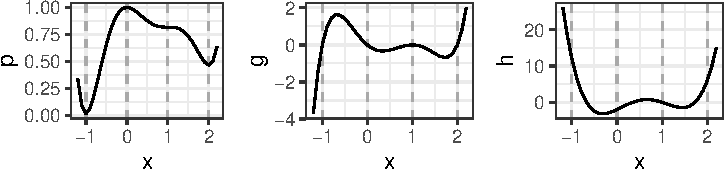
\includegraphics{RJ-2023-090_files/figure-latex/calculus-1.pdf}
\caption{\label{fig:calculus}Left: A polynomial. Center: First derivative (the gradient). Right: Second derivative (the Hessian).}
\end{figure}

\hypertarget{statistics-examples}{%
\section{Statistics examples}\label{statistics-examples}}

In this section we examine larger statistical examples and
demonstrate how \texttt{caracas} can help improve understanding of the models.

\hypertarget{example-linear-models}{%
\subsection{Example: Linear models}\label{example-linear-models}}

While the matrix form of linear models is quite clear and concise,
it can also be argued that matrix algebra
obscures what is being computed. Numerical examples are useful for
some aspects of the computations but not for others. In this respect
symbolic computations can be enlightening.

Consider a two-way analysis of variance (ANOVA) with one observation
per group, see Table \ref{tab:anova-two-way-table}.

\begin{table}[!h]
\centering
\caption{\label{tab:anova-two-way-table}Two-by-two layout of data.}
\centering
\begin{tabular}[t]{|>{}l|>{}l|}
\hline
$y_{11}$ & $y_{12}$\\
\hline
$y_{21}$ & $y_{22}$\\
\hline
\end{tabular}
\end{table}

Previously, it was demonstrated that a symbolic
vector could be defined with the \texttt{vector\_sym()} function.
Another way to specify a symbolic vector with explicit elements is
by using \texttt{as\_sym()}:

\begin{verbatim}
R> y  <- as_sym(c("y_11", "y_21", "y_12", "y_22"))
R> dat <- expand.grid(r = factor(1:2), s = factor(1:2))
R> X <- model.matrix(~ r + s, data = dat) |> as_sym()
R> b <- vector_sym(ncol(X), "b")
R> mu <- X %*% b
\end{verbatim}

For the specific model we have random variables \(y=(y_{ij})\). All
\(y_{ij}\)s are assumed independent and \(y_{ij}\sim N(\mu_{ij}, v)\).
The corresponding mean vector \(\mu\) has the form given below:

\begin{equation}
y = \left[\begin{matrix}y_{11}\\y_{21}\\y_{12}\\y_{22}\end{matrix}\right]; \quad X=\left[\begin{matrix}1 & . & .\\1 & 1 & .\\1 & . & 1\\1 & 1 & 1\end{matrix}\right]; \quad b=\left[\begin{matrix}b_{1}\\b_{2}\\b_{3}\end{matrix}\right]; \quad  \mu = X b = \left[\begin{matrix}b_{1}\\b_{1} + b_{2}\\b_{1} + b_{3}\\b_{1} + b_{2} + b_{3}\end{matrix}\right] .
\end{equation}

Above and elsewhere, dots represent zero.
The least squares estimate of \(b\) is the vector \(\hat{b}\) that minimizes \(||y-X b||^2\) which leads to the normal equations \((X^\top X)b = X^\top y\) to be solved. If \(X\) has full rank, the unique solution to the normal
equations is \(\hat{b} = (X^\top X)^{-1} X^\top y\). Hence the
estimated mean vector is \(\hat \mu = X\hat{b}=X(X^\top X)^{-1} X^\top y\). Symbolic computations are
not needed for quantities involving only the model matrix \(X\), but
when it comes to computations involving \(y\), a symbolic treatment of
\(y\) is useful:

\begin{verbatim}
R> Xty <- t(X) %*% y
R> b_hat <- solve(t(X) %*% X, Xty)
\end{verbatim}

\begin{align}
X^\top y &= \left[\begin{matrix}y_{11} + y_{12} + y_{21} + y_{22}\\y_{21} + y_{22}\\y_{12} + y_{22}\end{matrix}\right]; \quad 
\quad
\hat{b} = \frac{1}{2}  \left[\begin{matrix}\frac{3 y_{11}}{2} + \frac{y_{12}}{2} + \frac{y_{21}}{2} - \frac{y_{22}}{2}\\- y_{11} - y_{12} + y_{21} + y_{22}\\- y_{11} + y_{12} - y_{21} + y_{22}\end{matrix}\right].
\end{align}

Hence \(X^\top y\) (a sufficient reduction of data if the variance is
known) consists of the sum of all observations, the sum of
observations in the second row and the sum of observations in the
second column. For \(\hat{b}\), the second component is, apart from a
scaling, the sum of the second row minus the sum of the first
row. Likewise, the third component is the sum of the second column
minus the sum of the first column. Hence, for example the second
component of \(\hat{b}\) is the difference in mean between the first and
second column in Table \ref{tab:anova-two-way-table}.

\hypertarget{example-logistic-regression}{%
\subsection{Example: Logistic regression}\label{example-logistic-regression}}

In the following we go through details of the logistic regression model,
for a classical description see e.g. McCullagh and Nelder (1989) for a classical description.

As an example, consider the \texttt{budworm} data from the \CRANpkg{doBy} package (Højsgaard and Halekoh 2023).
The data shows the number of killed moth tobacco budworm
\emph{Heliothis virescens}. Batches of 20 moths of each sex were
exposed for three days to the pyrethroid and the number in each batch
that were dead or knocked down was recorded.
Below we focus only on male budworms and the mortality is illustrated
in Figure \ref{fig:budworm} (produced with \CRANpkg{ggplot2}; Wickham (2016)). The \(y\)-axis shows the empirical
logits, i.e.~\(\log((\texttt{ndead} + 0.5)/(\texttt{ntotal}-\texttt{ndead} + 0.5))\). The figure suggests that log odds of dying grows linearly with log dose.

\begin{verbatim}
R> data(budworm, package = "doBy")
R> bud <- subset(budworm, sex == "male")
R> bud
\end{verbatim}

\begin{verbatim}
#>    sex dose ndead ntotal
#> 1 male    1     1     20
#> 2 male    2     4     20
#> 3 male    4     9     20
#> 4 male    8    13     20
#> 5 male   16    18     20
#> 6 male   32    20     20
\end{verbatim}

\begin{figure}
\centering
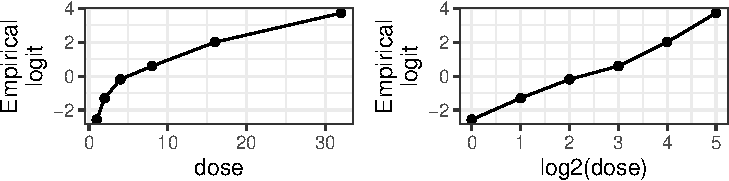
\includegraphics{RJ-2023-090_files/figure-latex/budworm-1.pdf}
\caption{\label{fig:budworm}Insecticide mortality of the moth tobacco budworm.}
\end{figure}

Observables are binomially distributed, \(y_i \sim \text{bin}(p_i, n_i)\). The probability \(p_i\) is connected to a \(q\)-vector of
covariates \(x_i=(x_{i1}, \dots, x_{iq})\) and a \(q\)-vector of
regression coefficients \(b=(b_1, \dots, b_q)\) as follows: The term
\(s_i = x_i \cdot b\) is denoted the \emph{linear predictor}. The
probability \(p_i\) can be linked to \(s_i\) in different ways, but the
most commonly employed is via the \emph{logit link function} which is
\(\text{logit}(p_i) = \log(p_i/(1-p_i))\) so here \(\text{logit}(p_i) = s_i\). Based on Figure \ref{fig:budworm}, we consider the specific
model with \(s_i = b_1 + b_2 \log2(dose_i)\). For later use, we define the data matrix below:

\begin{verbatim}
R> DM <- cbind(model.matrix(~log2(dose), data=bud),
+             bud[, c("ndead", "ntotal")])  |> as.matrix()
R> DM |> head(3)
\end{verbatim}

\begin{verbatim}
#>   (Intercept) log2(dose) ndead ntotal
#> 1           1          0     1     20
#> 2           1          1     4     20
#> 3           1          2     9     20
\end{verbatim}

\hypertarget{each-component-of-the-likelihood}{%
\subsubsection{Each component of the likelihood}\label{each-component-of-the-likelihood}}

The log-likelihood is \(\log L=\sum_i y_i \log(p_i) + (n_i-y_i) \log(1-p_i) = \sum_i \log L_i\), say.
Consider the contribution to the total log-likelihood from the \(i\)th
observation which is \(\log L_i = l_i = y_i \log(p_i) + (n_i-y_i) \log(1-p_i)\).
Since we are focusing on one observation only, we shall ignore the
subscript \(i\) in this section. First notice that with
\(s = \log(p/(1-p))\) we can find \(p\) as a function of \(s\) as:

\begin{verbatim}
R> def_sym(s, p) # The previous polynomial p is removed by this new declaration
R> sol_ <- solve_sys(lhs = log(p / (1 - p)), rhs = s, vars = p)
R> p_s <- sol_[[1]]$p
\end{verbatim}

\begin{equation}
\texttt{p\_s} = \frac{e^{s}}{e^{s} + 1}
\end{equation}

Next, find the likelihood as a function of \(p\), as a function of \(s\)
and as a function of \(b\). The underscore in \texttt{logLb\_} and elsewhere
indicates that this expression is defined in terms of other
symbols. The log-likelihood can be maximized using e.g.~Newton-Raphson
(see e.g. Nocedal and Wright (2006)) and in this connection we need the score function,
\(S\), and the Hessian, \(H\):

\begin{verbatim}
R> def_sym(y, n)
R> b  <- vector_sym(2, "b")
R> x  <- vector_sym(2, "x")
R> logLp_ <- y * log(p) + (n - y) * log(1 - p) # logL as fn of p
R> s_b <- sum(x * b)                           # s as fn of b
R> p_b <- subs(p_s, s, s_b)                    # p as fn of b
R> logLb_ <- subs(logLp_, p, p_b)              # logL as fn of b
R> Sb_ <- score(logLb_, b) |> simplify()
R> Hb_ <- hessian(logLb_, b) |> simplify()
\end{verbatim}

\begin{align}
\texttt{p\_b}   &= \frac{e^{b_{1} x_{1} + b_{2} x_{2}}}{e^{b_{1} x_{1} + b_{2} x_{2}} + 1}; \\
\texttt{logLb}\_ &= y \log{\left(\frac{e^{b_{1} x_{1} + b_{2} x_{2}}}{e^{b_{1} x_{1} + b_{2} x_{2}} + 1} \right)} + \left(n - y\right) \log{\left(1 - \frac{e^{b_{1} x_{1} + b_{2} x_{2}}}{e^{b_{1} x_{1} + b_{2} x_{2}} + 1} \right)}; \\
\texttt{Sb}\_    &= \left[\begin{matrix}\frac{x_{1} \left(- n e^{b_{1} x_{1} + b_{2} x_{2}} + y e^{b_{1} x_{1} + b_{2} x_{2}} + y\right)}{e^{b_{1} x_{1} + b_{2} x_{2}} + 1}\\\frac{x_{2} \left(- n e^{b_{1} x_{1} + b_{2} x_{2}} + y e^{b_{1} x_{1} + b_{2} x_{2}} + y\right)}{e^{b_{1} x_{1} + b_{2} x_{2}} + 1}\end{matrix}\right]; \\
\texttt{Hb}\_    &= \left[\begin{matrix}- \frac{n x_{1}^{2} e^{b_{1} x_{1} + b_{2} x_{2}}}{2 e^{b_{1} x_{1} + b_{2} x_{2}} + e^{2 b_{1} x_{1} + 2 b_{2} x_{2}} + 1} & - \frac{n x_{1} x_{2} e^{b_{1} x_{1} + b_{2} x_{2}}}{2 e^{b_{1} x_{1} + b_{2} x_{2}} + e^{2 b_{1} x_{1} + 2 b_{2} x_{2}} + 1}\\- \frac{n x_{1} x_{2} e^{b_{1} x_{1} + b_{2} x_{2}}}{2 e^{b_{1} x_{1} + b_{2} x_{2}} + e^{2 b_{1} x_{1} + 2 b_{2} x_{2}} + 1} & - \frac{n x_{2}^{2} e^{b_{1} x_{1} + b_{2} x_{2}}}{2 e^{b_{1} x_{1} + b_{2} x_{2}} + e^{2 b_{1} x_{1} + 2 b_{2} x_{2}} + 1}\end{matrix}\right] . 
\end{align}

There are some possible approaches before
maximizing the total log likelihood. One is to insert data case by
case into the symbolic log likelihood:

\begin{verbatim}
R> nms <- c("x1", "x2", "y", "n")
R> DM_lst <- doBy::split_byrow(DM)
R> logLb_lst <- lapply(DM_lst, function(vls) {
+     subs(logLb_, nms, vls)
+ })
\end{verbatim}

For example, the contribution from the third observation to the total log likelihood is:

\begin{align}
\texttt{logLb\_lst[[3]]}  &= 9 \log{\left(\frac{e^{b_{1} + 2 b_{2}}}{e^{b_{1} + 2 b_{2}} + 1} \right)} + 11 \log{\left(1 - \frac{e^{b_{1} + 2 b_{2}}}{e^{b_{1} + 2 b_{2}} + 1} \right)}.
\end{align}

The full likelihood can be maximized either e.g.~
using SymPy (not pursued here) or by converting the sum to an R
function which can be maximized using one of R's internal
optimization procedures:

\begin{verbatim}
R> logLb_tot <- Reduce(`+`, logLb_lst) 
R> logLb_fn  <- as_func(logLb_tot, vec_arg = TRUE)
R> opt <- optim(c(b1 = 0, b2 = 0), logLb_fn, 
+               control = list(fnscale = -1), hessian = TRUE)
R> opt$par
\end{verbatim}

\begin{verbatim}
#>    b1    b2 
#> -2.82  1.26
\end{verbatim}

The same model can be fitted e.g.~using R's \texttt{glm()} function as follows:

\begin{verbatim}
R> m <- glm(cbind(ndead, ntotal - ndead) ~ log2(dose), family=binomial(), data=bud)
R> m |> coef()
\end{verbatim}

\begin{verbatim}
#> (Intercept)  log2(dose) 
#>       -2.82        1.26
\end{verbatim}

\hypertarget{the-total-likelihood-symbolically}{%
\subsubsection{The total likelihood symbolically}\label{the-total-likelihood-symbolically}}

We conclude this section by illustrating that the log-likelihood for the entire dataset
can be constructed in a few steps (output is omitted to save space):

\begin{verbatim}
R> N <- 6; q <- 2
R> X <- matrix_sym(N, q, "x")
R> n <- vector_sym(N, "n")
R> y <- vector_sym(N, "y")
R> p <- vector_sym(N, "p")
R> s <- vector_sym(N, "s")
R> b <- vector_sym(q, "b")
\end{verbatim}

\begin{equation}
 X=\left[\begin{matrix}x_{11} & x_{12}\\x_{21} & x_{22}\\x_{31} & x_{32}\\x_{41} & x_{42}\\x_{51} & x_{52}\\x_{61} & x_{62}\end{matrix}\right]; \quad
 n=\left[\begin{matrix}n_{1}\\n_{2}\\n_{3}\\n_{4}\\n_{5}\\n_{6}\end{matrix}\right]; \quad
 y=\left[\begin{matrix}y_{1}\\y_{2}\\y_{3}\\y_{4}\\y_{5}\\y_{6}\end{matrix}\right] .
\end{equation}

The symbolic computations are as follows: We express the linear predictor \(s\) as function of the regression coefficients \(b\) and express the probability \(p\) as function of the linear predictor:

\begin{verbatim}
R> logLp <- sum(y * log(p) + (n - y) * log(1 - p)) # logL as fn of p
R> p_s <- exp(s) / (exp(s) + 1)                    # p as fn of s
R> s_b <- X %*% b                                  # s as fn of b
R> p_b <- subs(p_s, s, s_b)                        # p as fn of b
R> logLb_ <- subs(logLp, p, p_b)                   # logL as fn of b
\end{verbatim}

Next step could be to go from symbolic to numerical computations by
inserting numerical values. From here, one may proceed by computing
the score function and the Hessian matrix and solve the score
equation, using e.g.~Newton-Raphson. Alternatively, one might create an
R function based on the log-likelihood, and maximize this function
using one of R's optimization methods (see the example in the
previous section):

\begin{verbatim}
R> logLb <- subs(logLb_, cbind(X, y, n), DM)
R> logLb_fn <- as_func(logLb, vec_arg = TRUE)
R> opt <- optim(c(b1 = 0, b2 = 0), logLb_fn, 
+               control = list(fnscale = -1), hessian = TRUE)
R> opt$par
\end{verbatim}

\begin{verbatim}
#>    b1    b2 
#> -2.82  1.26
\end{verbatim}

\hypertarget{example-constrained-maximum-likelihood}{%
\subsection{Example: Constrained maximum likelihood}\label{example-constrained-maximum-likelihood}}

In this section we illustrate constrained optimization using Lagrange multipliers.
This is demonstrated for the independence model for a two-way contingency table.
Consider a \(2 \times 2\) contingency table with cell
counts \(y_{ij}\) and cell probabilities \(p_{ij}\) for \(i=1,2\) and \(j=1,2\),
where \(i\) refers to row and \(j\) to column as
illustrated in Table \ref{tab:anova-two-way-table}.

Under multinomial sampling, the log likelihood is

\begin{equation}
 l = \log L = \sum_{ij} y_{ij} \log(p_{ij}).
\end{equation}

Under the assumption of independence between rows and columns, the cell
probabilities have the form, (see e.g. Højsgaard, Edwards, and Lauritzen (2012), p.~32)

\begin{equation}
p_{ij}=u \cdot r_i \cdot s_j.
\end{equation}

To make the parameters \((u, r_i, s_j)\) identifiable, constraints
must be imposed. One possibility is to require that \(r_1=s_1=1\). The
task is then to estimate \(u\), \(r_2\), \(s_2\) by maximizing the log likelihood
under the constraint that \(\sum_{ij} p_{ij} = 1\). These constraints
can be
imposed using a Lagrange multiplier where we solve the
unconstrained optimization problem \(\max_p Lag(p)\) where
\begin{align}
  Lag(p) &= -l(p) + \lambda g(p) \quad \text{under the constraint that} \\
  g(p) &= \sum_{ij} p_{ij} - 1 = 0 ,
\end{align}
where \(\lambda\) is a Lagrange multiplier.
The likelihood equations can be found in closed-form.
In SymPy, \texttt{lambda} is a reserved symbol so it is denoted by an postfixed underscore below:

\begin{verbatim}
R> def_sym(u, r2, s2, lambda_)
R> y  <- as_sym(c("y_11", "y_21", "y_12", "y_22"))
R> p  <- as_sym(c("u", "u*r2", "u*s2", "u*r2*s2"))
R> logL <- sum(y * log(p))
R> Lag  <- -logL + lambda_ * (sum(p) - 1) 
R> vars <- list(u, r2, s2, lambda_)
R> gLag <- der(Lag, vars)
R> sol  <- solve_sys(gLag, vars)
R> print(sol, method = "ascii")
\end{verbatim}

\begin{verbatim}
#> Solution 1:
#>   lambda_ =  y_11 + y_12 + y_21 + y_22 
#>   r2      =  (y_21 + y_22)/(y_11 + y_12) 
#>   s2      =  (y_12 + y_22)/(y_11 + y_21) 
#>   u       =  (y_11 + y_12)*(y_11 + y_21)/(y_11 + y_12 + y_21 + y_22)^2
\end{verbatim}

\begin{verbatim}
R> sol <- sol[[1]]
\end{verbatim}

There is only one critical point. The fitted cell probabilities \(\hat p_{ij}\) are:

\begin{verbatim}
R> p11 <- sol$u
R> p21 <- sol$u * sol$r2
R> p12 <- sol$u * sol$s2
R> p22 <- sol$u * sol$r2 * sol$s2
R> p.hat <- matrix_(c(p11, p21, p12, p22), nrow = 2)
\end{verbatim}

\begin{equation}
\hat p = \frac{1}{\left(y_{11} + y_{12} + y_{21} + y_{22}\right)^{2}}  \left[\begin{matrix}\left(y_{11} + y_{12}\right) \left(y_{11} + y_{21}\right) & \left(y_{11} + y_{12}\right) \left(y_{12} + y_{22}\right)\\\left(y_{11} + y_{21}\right) \left(y_{21} + y_{22}\right) & \left(y_{12} + y_{22}\right) \left(y_{21} + y_{22}\right)\end{matrix}\right]
\end{equation}

To verify that the maximum likelihood estimate has been found, we compute the Hessian matrix
which is negative definite (the Hessian matrix is diagonal so the eigenvalues are the diagonal entries and these are all negative), output omitted:

\begin{verbatim}
R> H <- hessian(logL, list(u, r2, s2)) |> simplify()
\end{verbatim}

\hypertarget{example-an-auto-regression-model}{%
\subsection{Example: An auto regression model}\label{example-an-auto-regression-model}}

\hypertarget{symbolic-computations}{%
\subsubsection{Symbolic computations}\label{symbolic-computations}}

In this section we study the auto regressive model of order \(1\) (an AR(1) model, see
e.g. Shumway and Stoffer (2016), p.~75):
Consider random variables \(x_1, x_2, \dots, x_n\) following a stationary zero mean AR(1) process:

\begin{equation}
  x_i = a x_{i-1} + e_i; \quad i=2, \dots, n,
  \label{eq:ar1}
\end{equation}

where \(e_i \sim N(0, v)\) and all independent and with constant variance \(v\).
The marginal distribution of \(x_1\) is also assumed normal, and for the process to be stationary
we must have that the variance \(\mathbf{Var}(x_1) = v / (1-a^2)\).
Hence we can write \(x_1 = \frac 1 {\sqrt{1-a^2}} e_1\).

For simplicity of exposition, we set \(n=4\) such that \(e=(e_1, \dots, e_4)\) and \(x=(x_1, \dots x_4)\). Hence \(e \sim N(0, v I)\). Isolating
error terms in \eqref{eq:ar1} gives

\begin{equation}
  e= \left[\begin{matrix}e_{1}\\e_{2}\\e_{3}\\e_{4}\end{matrix}\right] = \left[\begin{matrix}\sqrt{1 - a^{2}} & . & . & .\\- a & 1 & . & .\\. & - a & 1 & .\\. & . & - a & 1\end{matrix}\right] \left[\begin{matrix}x_{1}\\x_{2}\\x_{3}\\x_{4}\end{matrix}\right] = L x  .
\end{equation}

Since
\(\mathbf{Var}(e)=v I\) we have \(\mathbf{Var}(e)=v I=L \mathbf{Var}(x) L^\top\) so the covariance matrix of \(x\) is \(V=\mathbf{Var}(x) = v L^{-1} \left (L^{-1} \right )^\top\) while the concentration matrix (the inverse covariance
matrix) is \(K=v^{-1}L^\top L\):

\begin{verbatim}
R> def_sym(a, v)
R> n <- 4
R> L <- diff_mat(n, "-a") # The difference matrix, L, shown above
R> L[1, 1] <- sqrt(1 - a^2)
R> Linv <- solve(L)
R> K <- crossprod_(L) / v
R> V <- tcrossprod_(Linv) * v
\end{verbatim}

\begin{align} 
    L^{-1} &= \left[\begin{matrix}\frac{1}{\sqrt{1 - a^{2}}} & . & . & .\\\frac{a}{\sqrt{1 - a^{2}}} & 1 & . & .\\\frac{a^{2}}{\sqrt{1 - a^{2}}} & a & 1 & .\\\frac{a^{3}}{\sqrt{1 - a^{2}}} & a^{2} & a & 1\end{matrix}\right] ; \\ 
    K &= \frac{1}{v}  \left[\begin{matrix}1 & - a & 0 & 0\\- a & a^{2} + 1 & - a & 0\\0 & - a & a^{2} + 1 & - a\\0 & 0 & - a & 1\end{matrix}\right] ; \\ 
    V &= \frac{v}{a^{2} - 1}  \left[\begin{matrix}-1 & - a & - a^{2} & - a^{3}\\- a & -1 & - a & - a^{2}\\- a^{2} & - a & -1 & - a\\- a^{3} & - a^{2} & - a & -1\end{matrix}\right]  .
  \end{align}

The zeros in the concentration matrix \(K\) implies a conditional
independence restriction: If the \(ij\)th element of a concentration
matrix is zero then \(x_i\) and \(x_j\) are conditionally independent
given all other variables (see e.g. Højsgaard, Edwards, and Lauritzen (2012), p.~84 for
details).

Next, we take the step from symbolic computations to numerical
evaluations. The joint distribution of \(x\) is multivariate normal
distribution, \(x\sim N(0, K^{-1})\). Let \(W=x x^\top\) denote the
matrix of (cross) products. The log-likelihood is therefore (ignoring
additive constants)

\begin{equation}
\log L = \frac n 2 (\log \mathbf{det}(K) - x^\top K x) = \frac n 2 (\log \mathbf{det}(K) - \mathbf{tr}(K W)), 
\end{equation}

where we note that \(\mathbf{tr}(KW)\) is the
sum of the elementwise products of \(K\) and \(W\) since both matrices are
symmetric. Ignoring the constant \(\frac n 2\),
this can be written symbolically to obtain the expression in
this particular case:

\begin{verbatim}
R> x <- vector_sym(n, "x")
R> logL <- log(det(K)) - sum(K * (x %*% t(x))) |> simplify()
\end{verbatim}

\begin{equation}
\log L = \log{\left(- \frac{a^{2}}{v^{4}} + \frac{1}{v^{4}} \right)} - \frac{- 2 a x_{1} x_{2} - 2 a x_{2} x_{3} - 2 a x_{3} x_{4} + x_{1}^{2} + x_{2}^{2} \left(a^{2} + 1\right) + x_{3}^{2} \left(a^{2} + 1\right) + x_{4}^{2}}{v} .
\end{equation}

\hypertarget{numerical-evaluation}{%
\subsubsection{Numerical evaluation}\label{numerical-evaluation}}

Next we illustrate how bridge the gap from symbolic computations to numerical computations based on a dataset:
For a specific data vector we get:

\begin{verbatim}
R> xt <- c(0.1, -0.9, 0.4, 0.0)
R> logL. <- subs(logL, x, xt) 
\end{verbatim}

\begin{equation}
\log L = \log{\left(- \frac{a^{2}}{v^{4}} + \frac{1}{v^{4}} \right)} - \frac{0.97 a^{2} + 0.9 a + 0.98}{v} .
\end{equation}

We can use R for numerical maximization of the likelihood and constraints on the
parameter values can be imposed e.g.~in the \texttt{optim()} function:

\begin{verbatim}
R> logL_wrap <- as_func(logL., vec_arg = TRUE)
R> eps <- 0.01
R> par <- optim(c(a=0, v=1), logL_wrap, 
+              lower=c(-(1-eps), eps), upper=c((1-eps), 10),
+              method="L-BFGS-B", control=list(fnscale=-1))$par
R> par
\end{verbatim}

\begin{verbatim}
#>      a      v 
#> -0.376  0.195
\end{verbatim}

The same model can be fitted e.g.~using R's \texttt{arima()} function as follows (output omitted):

\begin{verbatim}
R> arima(xt, order = c(1, 0, 0), include.mean = FALSE, method = "ML")
\end{verbatim}

It is less trivial to do the optimization in \texttt{caracas} by solving the score equations.
There are some possibilities for putting assumptions on variables
in \texttt{caracas} (see the ``Reference'' vignette), but
it is not possible to restrict the parameter \(a\) to only take values in \((-1, 1)\).

\hypertarget{example-variance-of-average-of-correlated-variables}{%
\subsection{Example: Variance of average of correlated variables}\label{example-variance-of-average-of-correlated-variables}}

Consider random
variables \(x_1,\dots, x_n\) where \(\mathbf{Var}(x_i)=v\) and \(\mathbf{Cov}(x_i, x_j)=v r\) for \(i\not = j\), where \(0 \le |r| \le1\).
For \(n=3\), the covariance matrix of \((x_1,\dots, x_n)\) is therefore

\begin{equation}
  \label{eq:1}
  V = v R = v \left[\begin{matrix}1 & r & r\\r & 1 & r\\r & r & 1\end{matrix}\right]. 
\end{equation}

Let \(\bar x = \sum_i x_i / n\) denote the average. Suppose interest is
in the variance of the average, \(w_{nr}=\mathbf{Var}(\bar x)\), when \(n\) goes
to infinity. Here the
subscripts \(n\) and \(r\) emphasize the dependence on the sample size \(n\)
and the correlation \(r\).
The variance of a sum \(x. = \sum_i x_i\) is
\(\mathbf{Var}(x.) = \sum_i \mathbf{Var}(x_i) + 2 \sum_{ij:i<j} \mathbf{Cov}(x_i, x_j)\) (i.e., the sum of the elements of the
covariance matrix). Then \(w_{nr}=Var(\bar x) = Var(x.)/n^2\).
We can do this in \texttt{caracas} as follows using the \texttt{sum\_} function
that calculate a symbolic sum:

\begin{verbatim}
R> def_sym(v, r, n, j, i)
R> s1 <- sum_(r, j, i+1, n) # sum_{j = i+1}^n r
R> s2 <- sum_(s1, i, 1, n-1) |> simplify()
R> var_sum <- v*(n + 2 * s2) |> simplify()
R> w_nr <- var_sum / n^2
\end{verbatim}

Above, \texttt{s1} is the sum of elements \(i+1\) to \(n\) in row \(j\) of the covariance matrix
and therefore \texttt{s2} is the sum of the entire upper triangular of the covariance matrix.

\begin{align}
\texttt{s1} &= r \left(- i + n\right); \quad
\texttt{s2} = \frac{n r \left(n - 1\right)}{2}; \quad 
w_{nr} = \mathbf{Var}(\bar x)= \frac{v \left(r \left(n - 1\right) + 1\right)}{n}.
\end{align}

The limiting behavior of the variance
\(w_{nr}\) can be studied in different situations (results shown later):

\begin{verbatim}
R> l_1 <- lim(w_nr, n, Inf)           # when sample size n goes to infinity
R> l_2 <- lim(w_nr, r, 0, dir = '+')  # when correlation r goes to zero
R> l_3 <- lim(w_nr, r, 1, dir = '-')  # when correlation r goes to one
\end{verbatim}

Moreover, for a given correlation
\(r\) it is instructive to investigate how many independent variables,
say \(k_{nr}\) the \(n\) correlated variables correspond to (in the sense of
giving the same variance of the average), because then \(k_{nr}\) can be seen as a
measure of the amount of information in data. We call \(k_{nr}\) the
effective sample size. Moreover, one might study how \(k_{nr}\) behaves
as function of \(n\) when \(n \rightarrow \infty\). That is we must (1)
solve \(v (1 + (n-1)r)/n = v/k_{nr}\) for \(k_{nr}\) and (2) find the limit \(k_r = \lim_{n\rightarrow\infty} k_{nr}\):

\begin{verbatim}
R> def_sym(k_n)
R> sol <- solve_sys(w_nr - v / k_n, k_n)
R> k_nr <- sol[[1]]$k_n                  # effective sample size
R> k_r <- lim(k_nr, n, Inf)
\end{verbatim}

The findings above are:

\begin{equation}
l_1 = \lim_{n\rightarrow\infty} w_{nr} = r v; \quad
l_2 = \lim_{r\rightarrow 0} w_{nr} = \frac{v}{n}; \quad
l_3 = \lim_{r\rightarrow 1} w_{nr} = v; \quad
k_{nr} = \frac{n}{n r - r + 1}; \quad 
k_r = \frac{1}{r} .
\end{equation}

It is illustrative to supplement the symbolic computations above with
numerical evaluations, which shows that even a moderate correlation
reduces the effective sample size substantially. In
Fig. \ref{fig:correlated}, this is illustrated for a wider range of
correlations and sample sizes.

\begin{verbatim}
R> dat <- expand.grid(r = c(.1, .2, .5), n = c(10, 50, 1000))
R> k_nr_fn <- as_func(k_nr)
R> dat$k_nr <- k_nr_fn(r = dat$r, n = dat$n)
R> dat$k_r <- 1 / dat$r
R> dat
\end{verbatim}

\begin{verbatim}
#>     r    n k_nr k_r
#> 1 0.1   10 5.26  10
#> 2 0.2   10 3.57   5
#> 3 0.5   10 1.82   2
#> 4 0.1   50 8.47  10
#> 5 0.2   50 4.63   5
#> 6 0.5   50 1.96   2
#> 7 0.1 1000 9.91  10
#> 8 0.2 1000 4.98   5
#> 9 0.5 1000 2.00   2
\end{verbatim}

\begin{figure}[h]
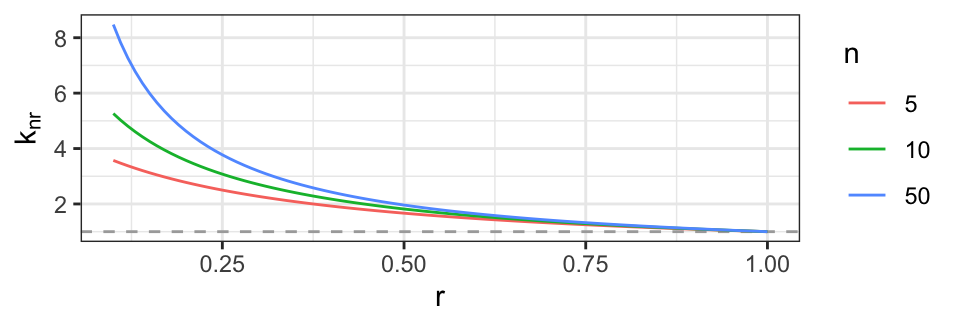
\includegraphics{RJ-2023-090_files/figure-latex/correlated-1} \caption{Effective sample size $k_{nr}$ as function of correlation $r$ for different values of $n$. The dashed line is the limit of $k_r$ as $r \rightarrow 1$, i.e. 1. }\label{fig:correlated}
\end{figure}

\hypertarget{further-topics}{%
\section{Further topics}\label{further-topics}}

\hypertarget{integration-limits-and-unevaluated-expressions}{%
\subsection{Integration, limits, and unevaluated expressions}\label{integration-limits-and-unevaluated-expressions}}

The unit circle is given by \(x^2 + y^2 = 1\) so the area of the upper
half of the unit circle is \(\int_{-1}^1 \sqrt{1-x^2}\; dx\) (which is
known to be \(\pi/2\)). This result is produced by \texttt{caracas} while the
\texttt{integrate} function in R produces the approximate result \(1.57\).

\begin{verbatim}
R> x <- as_sym("x")
R> half_circle_ <- sqrt(1 - x^2)
R> ad <- int(half_circle_, "x")          # Anti derivative
R> area <- int(half_circle_, "x", -1, 1) # Definite integral
\end{verbatim}

\begin{equation}
\texttt{ad} = \frac{x \sqrt{1 - x^{2}}}{2} + \frac{\operatorname{asin}{\left(x \right)}}{2}; \quad
\texttt{area} = \frac{\pi}{2}.
\end{equation}

Finally, we illustrate limits and the creation of unevaluated expressions:

\begin{verbatim}
R> def_sym(x, n)
R> y <- (1 + x/n)^n
R> l <- lim(y, n, Inf, doit = FALSE)
R> l_2 <- doit(l)
\end{verbatim}

\begin{equation}
l = \lim_{n \to \infty} \left(1 + \frac{x}{n}\right)^{n}; \quad l_2 = e^{x}
\end{equation}

Several functions have the \texttt{doit} argument, e.g.~\texttt{lim()}, \texttt{int()} and \texttt{sum\_()}.
Among other things, unevaluated expressions help making reproducible documents where the changes
in code appears automatically in the generated formulas.

\hypertarget{documents-with-mathematical-content}{%
\subsection{Documents with mathematical content}\label{documents-with-mathematical-content}}

A LaTeX rendering of a \texttt{caracas} symbol, say \texttt{x}, is obtained by typing
\texttt{\$\$x\ =\ \textasciigrave{}r\ tex(x)\textasciigrave{}\$\$}. This feature is useful
when creating documents with a mathematical content and has been used
extensively throughout this paper.

For rendering matrices, the \texttt{tex()} function
has a \texttt{zero\_as\_dot} argument which is useful:

\begin{verbatim}
R> A <- diag_(c("a", "b", "c"))
\end{verbatim}

\begin{equation}
\texttt{tex(A)} = \left[\begin{matrix}a & 0 & 0\\0 & b & 0\\0 & 0 & c\end{matrix}\right]; \quad \texttt{tex(A, zero\_as\_dot = TRUE)} = \left[\begin{matrix}a & . & .\\. & b & .\\. & . & c\end{matrix}\right]
\end{equation}

When displaying a matrix \(A\), the expression can sometimes be greatly
simplified by displaying \(k\) and \((A/k)\) for some factor \(k\). A specific
example could when displaying \(M^{-1}\). Here one may choose to display
\((1/det(M))\) and \(M^{-1} det(M)\). This can be illustrated as follows:

\begin{verbatim}
R> M0 <- toeplitz(c("a", "b"))  # Character matrix
R> M  <- as_sym(M0)             # as_sym() converts to a caracas symbol
R> Minv  <- solve(M)
R> Minv2 <- scale_matrix(Minv, det(Minv))
\end{verbatim}

\begin{equation}
\texttt{Minv} = \left[\begin{matrix}\frac{a}{a^{2} - b^{2}} & - \frac{b}{a^{2} - b^{2}}\\- \frac{b}{a^{2} - b^{2}} & \frac{a}{a^{2} - b^{2}}\end{matrix}\right]; \quad 
\texttt{Minv2} = \frac{1}{a^{2} - b^{2}}  \left[\begin{matrix}a & - b\\- b & a\end{matrix}\right]
\end{equation}

\hypertarget{extending-caracas}{%
\subsection{\texorpdfstring{Extending \texttt{caracas}}{Extending caracas}}\label{extending-caracas}}

It is possible to easily extend \texttt{caracas} with additional
functionality from SymPy using \texttt{sympy\_func()} from \texttt{caracas}
which we illustrate below. This example
illustrates how to use SymPy's \texttt{diff()} function to find univariate
derivatives multiple times. The partial derivative of \(\sin(xy)\)
with respect to \(x\) and \(y\) is found with \texttt{diff} in SymPy:

\begin{verbatim}
R> library(reticulate)
R> sympy <- import("sympy")
R> sympy$diff("sin(x * y)", "x", "y") 
\end{verbatim}

\begin{verbatim}
#> -x*y*sin(x*y) + cos(x*y)
\end{verbatim}

Alternatively:

\begin{verbatim}
R> x <- sympy$symbols("x")
R> y <- sympy$symbols("y")
R> sympy$diff(sympy$sin(x*y), x, y)
\end{verbatim}

One the other hand, the \texttt{der()} function in \texttt{caracas} finds the
gradient, which is a design choice in \texttt{caracas}:

\begin{verbatim}
R> def_sym(x, y)
R> f <- sin(x * y) 
R> der(f, list(x, y))
\end{verbatim}

\begin{verbatim}
#> c: [y*cos(x*y), x*cos(x*y)]
\end{verbatim}

If we want to obtain
the functionality from SymPy
we can write a function that invokes \texttt{diff} in SymPy using the
\texttt{sympy\_func()} function in \texttt{caracas}:

\begin{verbatim}
R> der_diff <- function(expr, ...) {
+    sympy_func(expr, "diff", ...)
+ }
R> der_diff(sin(x * y), x, y)
\end{verbatim}

\begin{verbatim}
#> c: -x*y*sin(x*y) + cos(x*y)
\end{verbatim}

This latter function is especially useful if we need to find the higher-order
derivative with respect to the same variable:

\begin{verbatim}
R> sympy$diff("sin(x * y)", "x", 100L)
R> der_diff(sin(x * y), x, 100L)
\end{verbatim}

\hypertarget{switching-back-and-forth-between-caracas-and-reticulate}{%
\subsection{\texorpdfstring{Switching back and forth between \texttt{caracas} and \texttt{reticulate}}{Switching back and forth between caracas and reticulate}}\label{switching-back-and-forth-between-caracas-and-reticulate}}

Another way of invoking SymPy functionality that is not available in
\texttt{caracas} is the following. As mentioned, a \texttt{caracas} symbol is a
list with a slot called \texttt{pyobj} (accessed by \texttt{\$pyobj}). Therefore, one can work with
\texttt{caracas} symbols in \texttt{reticulate}, and one can also coerce a Python
object into a \texttt{caracas} symbol. For example, it is straight forward
to create a Toeplitz matrix using \texttt{caracas}. The minor sub matrix
obtained by removing the first row and column using \texttt{reticulate} and
the result can be coerced to a \texttt{caracas} object with \texttt{as\_sym()},
e.g.~for numerical evaluation (introduced later).

\begin{verbatim}
R> A <- as_sym(toeplitz(c("a", "b", 0))) # caracas symbol
R> B_ <- A$pyobj$minor_submatrix(0, 1)   # reticulate object (notice: 0-based indexing)
R> B <- B_ |> as_sym()                   # caracas symbol
\end{verbatim}

\begin{equation}
A = \left[\begin{matrix}a & b & 0\\b & a & b\\0 & b & a\end{matrix}\right]; \quad
B = \left[\begin{matrix}b & b\\0 & a\end{matrix}\right].
\end{equation}

\hypertarget{hands-on-activities}{%
\section{Hands-on activities}\label{hands-on-activities}}

\begin{enumerate}
\def\labelenumi{\arabic{enumi}.}
\tightlist
\item
  Related to Section \protect\hyperlink{example-linear-models}{Example: Linear models}:

  \begin{enumerate}
  \def\labelenumii{\alph{enumii})}
  \tightlist
  \item
    The orthogonal projection
    matrix onto the span of the model matrix \(X\) is \(P=X (X^\top X)^{-1}X^\top\). The residuals are \(r=(I-P)y\). From this one may
    verify that these are not all independent.
  \item
    If one of the factors
    is ignored, then the two-way analysis of variance
    model becomes a one-way analysis of variance
    model, and it is illustrative to redo the computations in this setting.
  \item
    Likewise if an interaction between the two factors
    is included in the model, what are the residuals in this case?
  \end{enumerate}
\item
  Related to Section \protect\hyperlink{example-logistic-regression}{Example: Logistic regression}:

  \begin{enumerate}
  \def\labelenumii{\alph{enumii})}
  \tightlist
  \item
    In \protect\hyperlink{each-component-of-the-likelihood}{Each component of the
    likelihood}, Newton-Raphson can be implemented to solve the likelihood
    equations.
    Note how sensitive Newton-Raphson is to starting point.
    This can be solved by another optimisation scheme, e.g.~
    Nelder-Mead (optimising the log likelihood) or BFGS
    (finding extreme for the score function).
  \item
    The example is done as logistic regression with the logit
    link function. Try other link functions such as cloglog (complementary log-log).
  \end{enumerate}
\item
  Related to Section \protect\hyperlink{example-constrained-maximum-likelihood}{Example: Constrained maximum likelihood}:

  \begin{enumerate}
  \def\labelenumii{\alph{enumii})}
  \tightlist
  \item
    Identifiability of the parameters was handled by not including
    \(r_1\) and \(s_1\) in the specification of \(p_{ij}\). An alternative is
    to impose the restrictions \(r_1=1\) and \(s_1=1\), and this can also
    be handled via Lagrange multipliers. Another alternative is to regard
    the model as a log-linear model where \(\log p_{ij} = \log u + \log r_i + \log s_j = \tilde{u} + \tilde{r}_i + \tilde{s}_j\). This model
    is similar in its structure to the two-way ANOVA for Section \protect\hyperlink{example-linear-models}{Example: Linear
    models}. This model can be fitted as a generalized linear model
    with a Poisson likelihood and \(\log\) as link function. Hence, one
    may modify the results in Section \protect\hyperlink{example-logistic-regression}{Example: Logistic regression} to
    provide an alternative way of fitting the model.
  \item
    A simpler task is
    to consider a multinomial distribution with four categories,
    counts \(y_i\) and cell probabilities \(p_i\), \(i=1,2,3,4\) where \(\sum_i p_i=1\). For this model, find the maximum likelihood estimate for
    \(p_i\) (use the Hessian to verify that the critical point is a maximum).
  \end{enumerate}
\item
  Related to Section \protect\hyperlink{example-an-auto-regression-model}{Example: An auto regression model}:

  \begin{enumerate}
  \def\labelenumii{\alph{enumii})}
  \tightlist
  \item
    Compare the estimated parameter values with those obtained from
    the \texttt{arima()} function.
  \item
    Modify the model in Equation \eqref{eq:ar1} by
    setting \(x_1 = a x_n + e_1\) (``wrapping around'') and see what happens
    to the pattern of zeros in the concentration matrix.
  \item
    Extend the
    \(AR(1)\) model to an \(AR(2)\) model (``wrapping around'') and
    investigate this model along the same lines. Specifically,
    what are the conditional independencies (try at least \(n=6\))?
  \end{enumerate}
\item
  Related to Section \protect\hyperlink{example-variance-of-average-of-correlated-variables}{Example: Variance of average of correlated variables}:

  \begin{enumerate}
  \def\labelenumii{\alph{enumii})}
  \tightlist
  \item
    Simulate the situation given in the paper (e.g.~using the
    function \texttt{mvrnorm()} in R package \texttt{MASS})
    and verify that the results align with the symbolic computations.
  \item
    It is interesting to study such behaviours for other covariance
    functions.
    Replicate the calculations for the covariance matrix of the form
    \begin{equation}
      \label{eq:ex5}
      V = v R = v \left[\begin{matrix}1 & r & 0\\r & 1 & r\\0 & r & 1\end{matrix}\right],
    \end{equation}
    i.e., a special case of a Toeplitz matrix.
    How many independent variables, \(k\), do
    the \(n\) correlated variables correspond to?
  \end{enumerate}
\end{enumerate}

\hypertarget{discussion}{%
\section{Discussion}\label{discussion}}

We have presented the \texttt{caracas} package and argued that the
package extends the functionality of R significantly with respect to
symbolic mathematics.
In contrast to using \texttt{reticulate} and SymPy directly, \texttt{caracas}
provides symbolic mathematics in standard R syntax.

One practical virtue of \texttt{caracas} is
that the package integrates nicely with \texttt{Rmarkdown},
(J. Allaire et al. 2021), (e.g.~with the \texttt{tex()} functionality)\\
and thus supports creating of scientific documents and teaching
material. As for the usability in practice we await feedback from
users.

Another related R package is \texttt{Ryacas} based on Yacas (Pinkus and Winitzki 2002; Pinkus, Winnitzky, and Mazur 2016).
The \texttt{Ryacas} package has existed for many years and is still of relevance.
\texttt{Ryacas} probably has fewer features than \texttt{caracas}. On the other
hand, \texttt{Ryacas} does not require Python (it is compiled).
Finally, the Yacas language is extendable (see e.g.~the vignette
``User-defined yacas rules'' in the \texttt{Ryacas} package).

One possible future development could be an R package which is
designed without a view towards the underlying engine (SymPy or Yacas)
and which then draws more freely from SymPy and Yacas.
In this connection we mention that there are additional resources
on CRAN such as \CRANpkg{calculus} (Guidotti 2022).

Lastly, with respect to freely available resources in a CAS context, we would
like to draw attention to \texttt{WolframAlpha}, see e.g.~
\url{https://www.wolframalpha.com/}, which provides an online service for
answering (mathematical) queries.

\hypertarget{acknowledgements}{%
\section{Acknowledgements}\label{acknowledgements}}

We would like to thank the R Consortium for financial support for
creating the \texttt{caracas} package, users for pin pointing aspects
that can be improved in \texttt{caracas}
and Ege Rubak (Aalborg University, Denmark),
Poul Svante Eriksen (Aalborg University, Denmark),
Giovanni Marchetti (University of Florence, Italy)
and reviewers for constructive comments.

\hypertarget{references}{%
\section*{References}\label{references}}
\addcontentsline{toc}{section}{References}

\hypertarget{refs}{}
\begin{CSLReferences}{1}{0}
\leavevmode\vadjust pre{\hypertarget{ref-Allaire_Quarto_2022}{}}%
Allaire, J. J., Charles Teague, Carlos Scheidegger, Yihui Xie, and Christophe Dervieux. 2022. {``{Quarto}.''} \url{https://doi.org/10.5281/zenodo.5960048}.

\leavevmode\vadjust pre{\hypertarget{ref-rmarkdown}{}}%
Allaire, JJ, Yihui Xie, Jonathan McPherson, Javier Luraschi, Kevin Ushey, Aron Atkins, Hadley Wickham, Joe Cheng, Winston Chang, and Richard Iannone. 2021. \emph{Rmarkdown: Dynamic Documents for r}. \url{https://github.com/rstudio/rmarkdown}.

\leavevmode\vadjust pre{\hypertarget{ref-caracas:21}{}}%
Andersen, Mikkel Meyer, and Søren Højsgaard. 2021. {``{caracas: Computer algebra in R}.''} \emph{Journal of Open Source Software} 6 (63): 3438. \url{https://doi.org/10.21105/joss.03438}.

\leavevmode\vadjust pre{\hypertarget{ref-JSSv104i05}{}}%
Guidotti, Emanuele. 2022. {``{calculus: High-Dimensional Numerical and Symbolic Calculus in R}.''} \emph{Journal of Statistical Software} 104 (1): 1--37. \url{https://doi.org/10.18637/jss.v104.i05}.

\leavevmode\vadjust pre{\hypertarget{ref-hojsgaard}{}}%
Højsgaard, Søren, David Edwards, and Steffen Lauritzen. 2012. \emph{Graphical Models with {R}}. New York: Springer. \url{https://doi.org/10.1007/978-1-4614-2299-0}.

\leavevmode\vadjust pre{\hypertarget{ref-doBy}{}}%
Højsgaard, Søren, and Ulrich Halekoh. 2023. \emph{{doBy: Groupwise Statistics, LSmeans, Linear Estimates, Utilities}}. \url{https://github.com/hojsgaard/doby}.

\leavevmode\vadjust pre{\hypertarget{ref-mccullagh}{}}%
McCullagh, P, and John A Nelder. 1989. \emph{{Generalized Linear Models}}. 2nd ed. Chapman \& Hall/{CRC} Monographs on Statistics and Applied Probability. Philadelphia, PA: Chapman \& Hall/{CRC}. \url{https://www.routledge.com/Generalized-Linear-Models/McCullagh-Nelder/p/book/9780412317606}.

\leavevmode\vadjust pre{\hypertarget{ref-nocedal}{}}%
Nocedal, Jorge, and Stephen J. Wright. 2006. \emph{{Numerical Optimization}}. Springer New York. \url{https://doi.org/10.1007/978-0-387-40065-5}.

\leavevmode\vadjust pre{\hypertarget{ref-Pinkus2002}{}}%
Pinkus, Ayal, and Serge Winitzki. 2002. {``{YACAS: A Do-It-Yourself Symbolic Algebra Environment}.''} In \emph{Proceedings of the Joint International Conferences on Artificial Intelligence, Automated Reasoning, and Symbolic Computation}, 332--36. AISC '02/Calculemus '02. London, UK, UK: Springer-Verlag. \url{https://doi.org/10.1007/3-540-45470-5_29}.

\leavevmode\vadjust pre{\hypertarget{ref-yacas}{}}%
Pinkus, Ayal, Serge Winnitzky, and Grzegorz Mazur. 2016. {``{Yacas - Yet another computer algebra system}.''} \url{https://yacas.readthedocs.io/en/latest/}.

\leavevmode\vadjust pre{\hypertarget{ref-shumway:etal:16}{}}%
Shumway, Robert H., and David S. Stoffer. 2016. \emph{Time Series Analysis and Its Applications}. Fourth Edition. Springer. \url{https://doi.org/10.1007/978-3-319-52452-8}.

\leavevmode\vadjust pre{\hypertarget{ref-reticulate}{}}%
Ushey, Kevin, JJ Allaire, and Yuan Tang. 2020. \emph{Reticulate: Interface to 'Python'}. \url{https://CRAN.R-project.org/package=reticulate}.

\leavevmode\vadjust pre{\hypertarget{ref-ggplot2}{}}%
Wickham, Hadley. 2016. \emph{{g}gplot2: Elegant Graphics for Data Analysis}. Springer-Verlag New York. \url{https://ggplot2.tidyverse.org}.

\leavevmode\vadjust pre{\hypertarget{ref-RMarkdownDefinitiveGuide}{}}%
Xie, Yihui, J. J. Allaire, and Garrett Grolemund. 2018. \emph{R Markdown: The Definitive Guide}. Boca Raton, Florida: Chapman; Hall/{CRC}. \url{https://bookdown.org/yihui/rmarkdown}.

\leavevmode\vadjust pre{\hypertarget{ref-RMarkdownCookbook}{}}%
Xie, Yihui, Christophe Dervieux, and Emily Riederer. 2020. \emph{R Markdown Cookbook}. Boca Raton, Florida: Chapman; Hall/{CRC}. \url{https://bookdown.org/yihui/rmarkdown-cookbook}.

\end{CSLReferences}


\address{%
Mikkel Meyer Andersen\\
Department of Mathematical Sciences, Aalborg University, Denmark\\%
Skjernvej 4A\\ 9220 Aalborg Ø, Denmark\\
%
%
\textit{ORCiD: \href{https://orcid.org/0000-0002-0234-0266}{0000-0002-0234-0266}}\\%
\href{mailto:mikl@math.aau.dk}{\nolinkurl{mikl@math.aau.dk}}%
}

\address{%
Søren Højsgaard\\
Department of Mathematical Sciences, Aalborg University, Denmark\\%
Skjernvej 4A\\ 9220 Aalborg Ø, Denmark\\
%
%
\textit{ORCiD: \href{https://orcid.org/0000-0002-3269-9552}{0000-0002-3269-9552}}\\%
\href{mailto:sorenh@math.aau.dk}{\nolinkurl{sorenh@math.aau.dk}}%
}
